\documentclass[a4paper, 12pt]{article}%тип документа

%отступы
\usepackage[left=2cm,right=2cm,top=2cm,bottom=3cm,bindingoffset=0cm]{geometry}

%Русский язык
\usepackage[T2A]{fontenc} %кодировка
\usepackage[utf8]{inputenc} %кодировка исходного кода
\usepackage[english,russian]{babel} %локализация и переносы

%Вставка картинок
\usepackage{wrapfig}
\usepackage{graphicx}
\graphicspath{{pictures/}}
\DeclareGraphicsExtensions{.pdf,.png,.jpg}

%оглавление
\usepackage{titlesec}
\titlespacing{\chapter}{0pt}{-30pt}{12pt}
\titlespacing{\section}{\parindent}{5mm}{5mm}
\titlespacing{\subsection}{\parindent}{5mm}{5mm}
\usepackage{setspace}

%Графики
\usepackage{multirow}
\usepackage{pgfplots}
\pgfplotsset{compat=1.9}

%Математика
\usepackage{amsmath, amsfonts, amssymb, amsthm, mathtools}

%Стиль страницы
\usepackage{fancyhdr}
\pagestyle{fancy}

\begin{document}

\begin{titlepage}

\begin{center}
%\vspace*{1cm}
\large\textbf{Московский Физико-Технический Институт}\\
\large\textbf{(государственный университет)}
\vfill
\line(1,0){430}\\[1mm]
\huge\textbf{Работа 25}\\
\line(1,0){430}\\[1mm]
\vfill
\large Сибгатуллин Булат, ФРКТ\\
\end{center}

\end{titlepage}
\fancyhead[L] {Работа 25}
\noindent \textbf{Цель работы:} \\
\indent text\\
\noindent \textbf{В работе используются:} \\
\indent text

\section{Выполнение задания}

\subsection{Ознакомительные шаги}

\begin{enumerate}

\item Откроем в Micro-Cap файл adm3p.cir, в котором подготовлены схемы лестничных фильтров порядка \textit{n} = 3, реализующих входной адмиттанс.

\end{enumerate}

%Вставка изображения
%\begin{figure}[h!]
%\centering
%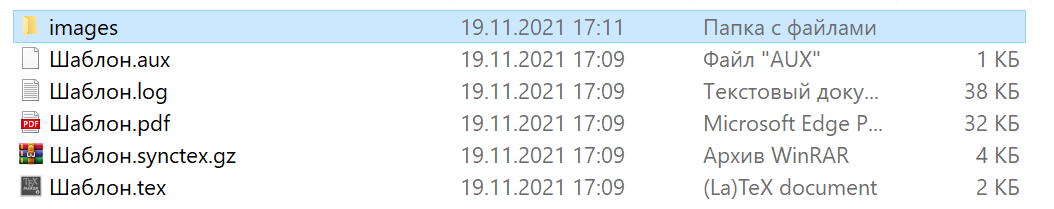
\includegraphics[scale=1]{images/image.png}
%\caption{text}
%\label{fig:Image1}
%\end{figure}

\subsection{Трехполюсные лестничные фильтры}

\begin{enumerate}

\item Откроем модель adm3p.cir и реализуем лестничные фильтры третьего порядка с параметрами:

\[R_0 = 50, \quad f_0 = 1MHz, \quad Q = 10.\]

Для этого вычислим эталонные значения:

\[L_0 = \frac{R_0}{2\pi f_0}, \quad C_0 = \frac{1}{2 \pi f_0 R_0}\]

и установим на схеме номиналы компонентов $f_0, Q, R_0, L_0, C_0$.

\item Сравним частотный характеристики фильтров с теоретическими, удостоверимся в правильности расчетов.

\item Сравним частотные характеристики по напряжению и по мощности. Измерим уровни затухания по мощности на границах полос пропускания, там где затухание по напряжению составляется 0.7. Запишем получившиеся данные в таблицу:

\begin{center}
\begin{tabular}{|c|c|c|c|c|}
\hline 
• & ФНЧ & ФВЧ & Полосовой & Режекторный \\ 
\hline 
Затухание по мощности & 0,5 & • & • & • \\ 
\hline 
\end{tabular} 
\end{center}

Исследуем степень деградации характеристик ... %тут дописать теорию

\begin{center}
\begin{tabular}{|c|c|c|c|c|}
\hline 
 & \multicolumn{2}{c|}{RSL} & \multicolumn{2}{c|}{RSL} \\ 
\hline 
 & Напряжение & Мощность & Напряжение & Мощность \\ 
\hline 
25 & 0,41 & 0,63 & 0,34 & 0,48 \\ 
\hline 
50 & 0,52 & 1 & 0,51 & 1 \\ 
\hline 
75 & 0,67 & 1,79 & 0,8 & 1,45 \\ 
\hline 
\end{tabular} 
\end{center}

\item Изучим фазовые характеристики фильтров, измерим значения фазовых сдвигов на нулевой и бесконечной частотах:

\begin{tabular}{|c|c|c|c|c|}
\hline 
 & ФНЧ & ФВЧ & Полосовой & Режекторный \\ 
\hline 
0 & 0 & • & • & • \\ 
\hline 
$\inf$ & $-\pi$ & • & • & • \\ 
\hline 
\end{tabular} 

\end{enumerate}

\end{document}